\documentclass[a4paper]{report}

%====================== PACKAGES ======================

\usepackage[utf8]{inputenc}
\usepackage[T1]{fontenc}
\usepackage[french]{babel}
%pour gérer les positionnement d'images
\usepackage{float}
\usepackage{amsmath, amsthm, amssymb}
\usepackage{amsfonts}
\usepackage{graphicx}
\usepackage[colorinlistoftodos]{todonotes}
\usepackage{url}
%pour les informations sur un document compilé en PDF et les liens externes / internes
\usepackage{hyperref}
%pour la mise en page des tableaux
\usepackage{array}
\usepackage{tabularx}
%pour utiliser \floatbarrier
%\usepackage{placeins}
%\usepackage{floatrow}
%espacement entre les lignes
\usepackage{setspace}
%modifier la mise en page de l'abstract
\usepackage{abstract}
%police et mise en page (marges) du document
\usepackage[T1]{fontenc}
\usepackage[top=2cm, bottom=2cm, left=2cm, right=2cm]{geometry}
%Pour les galerie d'images
\usepackage{subfig}
\usepackage{color}
\usepackage{array}
%pour les fonctions mathématiques et graphiques
\usepackage{gastex}
%\usepackage[dvips]{graphics}
\usepackage{pstricks}
\usepackage{a4wide}
\usepackage{multicol}
\usepackage{pst-tree}
\usepackage{tikz-qtree}
\usepackage{tikz}
\usetikzlibrary{arrows}
\tikzstyle{ent}=[circle,draw,thick,inner sep=0pt,minimum size=2.5mm]
\usetikzlibrary{arrows,automata,positioning}
\usetikzlibrary{automata,patterns,topaths,shapes,calc}
\tikzstyle{every picture}+=[>=stealth',initial text=]
\tikzstyle{state}=[rectangle,draw=black]
%liste de toutes les macros pour équations
\definecolor{OliveGreen}{rgb}{0,0.6,0}
\newcommand{\Q}{\mathbb{Q}}
\newcommand{\R}{\mathbb{R}}
\newcommand{\N}{\mathbb{N}}
\newcommand{\Z}{\mathbb{Z}}
\newcommand{\T}{\mathbb{T}}
\newcommand{\Bo}{\mathbb{B}}

\newcommand{\Au}{\mathcal{A}}
\newcommand{\B}{\mathcal{B}}
\newcommand{\C}{\mathcal{C}}
\newcommand{\D}{\mathcal{D}}
\newcommand{\F}{\mathcal{F}}
\newcommand{\G}{\mathcal{G}}
\newcommand{\K}{\mathcal{K}}
\newcommand{\Hr}{\mathcal{H}}
\newcommand{\I}{\mathcal{I}}
\newcommand{\La}{\mathcal{L}}
\newcommand{\M}{\mathcal{M}}
\newcommand{\Net}{\mathcal{N}}
\newcommand{\Pa}{\mathcal{P}}
\newcommand{\Rel}{\mathcal{R}}
\newcommand{\Sy}{\mathcal{S}}
\newcommand{\Ts}{\mathcal{T}}
\newcommand{\X}{\mathcal{X}}

\newcommand{\rel}{\bowtie}
\newcommand{\tr}{\xrightarrow}
\newcommand{\opeq}{\leftrightarrow}
\newcommand{\fee}{\varphi}
\newcommand{\eps}{\varepsilon}
\newcommand{\vect}[1]{\mathbf{#1}}
\newcommand{\fut}{\overrightarrow}
\newcommand\sui[1][a]{\ensuremath{\left(#1_n\right)_{n\in \N}}}

\newcommand{\E}{\textsf{E}}
\newcommand{\A}{\textsf{A}}

\DeclareMathOperator{\cla}{cl}

\theoremstyle{plain}

\newtheorem{theorem}{Théorème}
\newtheorem{lemma}[theorem]{Lemme}
\newtheorem{corollary}[theorem]{Corollaire}
\newtheorem{proposition}[theorem]{Proposition}

\newtheorem{definition}[theorem]{Définition}

\theoremstyle{remark}
\newtheorem{remark}[theorem]{Remarque}
\newtheorem{example}[theorem]{Exemple}

%====================== INFORMATION ET REGLES ======================

%rajouter les numérotation pour les \paragraphe et \subparagraphe
\setcounter{secnumdepth}{4}
\setcounter{tocdepth}{4}

\hypersetup{							% Information sur le document
pdfauthor = {Premier Auteur,
			Deuxième Auteur,
			Troisième Auteur,
    		Quatrième Auteur},			% Auteurs
pdftitle = {Nom du Projet -
			Sujet du Projet},			% Titre du document
pdfsubject = {Mémoire de Projet},		% Sujet
pdfkeywords = {Tag1, Tag2, Tag3, ...},	% Mots-clefs
pdfstartview={FitH}}					% ajuste la page à la largueur de l'écran
%pdfcreator = {MikTeX},% Logiciel qui a crée le document
%pdfproducer = {}} % Société avec produit le logiciel

%======================== DEBUT DU DOCUMENT ========================

\begin{document}

%régler l'espacement entre les lignes
\newcommand{\HRule}{\rule{\linewidth}{0.5mm}}

%page de garde
\begin{titlepage}
\begin{center}

% Upper part of the page. The '~' is needed because only works if a paragraph has started.

\includegraphics[width=0.35\textwidth]{./logo.png}~\\[1cm]

\textsc{\LARGE Université Pierre et Marie Curie}\\[1.5cm]

\textsc{\Large }\\[0.5cm]

% Title
\HRule \\[0.4cm]

{\huge \bfseries Projet PSAR\\
Une interface graphique pour la logique \\[0.4cm] }

\HRule \\[1.5cm]

% Author and supervisor
\begin{minipage}{0.4\textwidth}
\begin{flushleft} \large
\emph{Auteurs:}\\
Bastien \textsc{RIGAULT}\\
Sandra \textsc{LADURANTI}
\end{flushleft}
\end{minipage}
\begin{minipage}{0.4\textwidth}
\begin{flushright} \large
\emph{Référents:} \\
Béatrice \textsc{BERARD}\\
Mathieu \textsc{JAUME}\\
Bénédicte \textsc{LEGASTELOIS}\\
\end{flushright}
\end{minipage}

\vfill

% Bottom of the page
{\large \today}

\end{center}
\end{titlepage}

%page blanche
\newpage
~
%ne pas numéroter cette page
\thispagestyle{empty}
\newpage

\renewcommand{\abstractnamefont}{\normalfont\Large\bfseries}
%\renewcommand{\abstracttextfont}{\normalfont\Huge}

\begin{abstract}
\hskip7mm

\begin{spacing}{1.3}

L'objectif de ce projet, réalisé dans le cadre de l'UE PSAR (4I408)
est de concevoir un logiciel pédagogique pour l'apprentissage de la
logique du premier ordre. Ce logiciel apportera notamment un support
visuel sous la forme d'un jardin et de fleurs permettant d'appréhender
plus facilement les formules de la logique. Les étudiants auront à
leur disposition deux fenêtres : l'une permettant de concevoir un
jardin en y positionnant des fleurs et l'autre permettant d'écrire des
formules à l'aide d'un clavier visuel. Ils pourront alors soit
construire un jardin respectant un ensemble de formule données, ou au
contraire établir des formules à partir d'un jardin donné. Les
formules pourront être analysées de manière automatique afin de
vérifier leur cohérence. Enfin, les étudiants pourront sauvegarder
leurs jardins et leurs formules pour les réutiliser ultérieurement.
\newline
La première partie de ce rapport présente plus amplement le sujet, les outils mis à disposition pour le réaliser et les premières pistes pour résoudre les problématiques liées à leurs utilisation.
La seconde partie explique concrètement quels vont être les fonctionnalités à développer ainsi que l'organisation du travail dans le groupe et la structure général du code.
La partie suivante explore plus amplement les choix techniques qui ont été réalisé, leurs avantages et inconvénients ainsi que leurs utilisation et rôle dans la réalisation du projet.
Enfin, ce rapport se conclu sur une analyse des résultats obtenu en comparaison des attentes formulées dans le cahier des charges.

\end{spacing}
\end{abstract}


\tableofcontents
\thispagestyle{empty}
\setcounter{page}{0}
%ne pas numéroter le sommaire

\newpage

%espacement entre les lignes d'un tableau
\renewcommand{\arraystretch}{1.5}

%====================== INCLUSION DES PARTIES ======================

~
\thispagestyle{empty}
%recommencer la numérotation des pages à "1"
\setcounter{page}{0}
\newpage

\documentclass{beamer}

\usepackage[utf8]{inputenc}
\usepackage[french]{babel}
\usepackage[T1]{fontenc}
\usepackage{tikz}
\usetikzlibrary{shapes, arrows}

\usetheme{Montpellier}
%\usecolortheme{lily}

%STYLE
\tikzstyle{block} = [rectangle, draw, fill=blue!10,
	text width=5em, text centered, rounded corners, minimum width=100pt, minimum height=25pt]
\tikzstyle{cloud} = [draw, ellipse, fill=red!10, node distance=5cm, minimum height=2em]

\title{PSAR - Logika}
\author{Sandra \textsc{LADURANTI} et Bastien \textsc{RIGAULT}}
\date{2015-2016}
\begin{document}



	\begin{frame}
		
\includegraphics[width=0.20\textwidth]{logo}
		\titlepage
	\end{frame}
	
	\begin{frame}
		\frametitle{Sommaire}
		\tableofcontents
	\end{frame}
	
	\section{Architecture générale}
	\begin{frame}
	\begin{figure}
	\centering	
	
	
	\begin{tikzpicture}[node distance = 2cm, auto]
		%Place node		%Place node
		\node [block] (ui) {Interface graphique};
		\node [cloud, left of=ui] (uiAction) {Action utilisateur};
		\node [block, below of=ui] (ctrl) {Contrôleur};
		\node [cloud, left of=ctrl] (aig) {Aiguillage};
		\node [block, below of=ctrl] (mod) {Modèle};
		\node [cloud, left of=mod] (proc) {Traitement};
		
		%Draw edges
		\draw [->] (ui.-150) -- (ctrl.155);
		\draw [->] (ctrl.-130) -- (mod.130);
		\draw [->] (mod.50) -- (ctrl.-50);
		\draw [->] (ctrl.25) -- (ui.-30);
		
		\draw [->, dashed] (uiAction) -- (ui);
		\draw [->, dashed] (mod) -- (proc);
		\draw [->, dashed] (proc) -- (mod);
		
	\end{tikzpicture}
	\end{figure}
	\end{frame}
	
	\section{Exemple : Traitement d'une formule (1)}
	\begin{frame}
	\includegraphics[scale=0.4]{organisationProg}
	\end{frame}
	
	\section{Exemple : Traitement d'une formule (2)}
	\begin{frame}
	\centering
	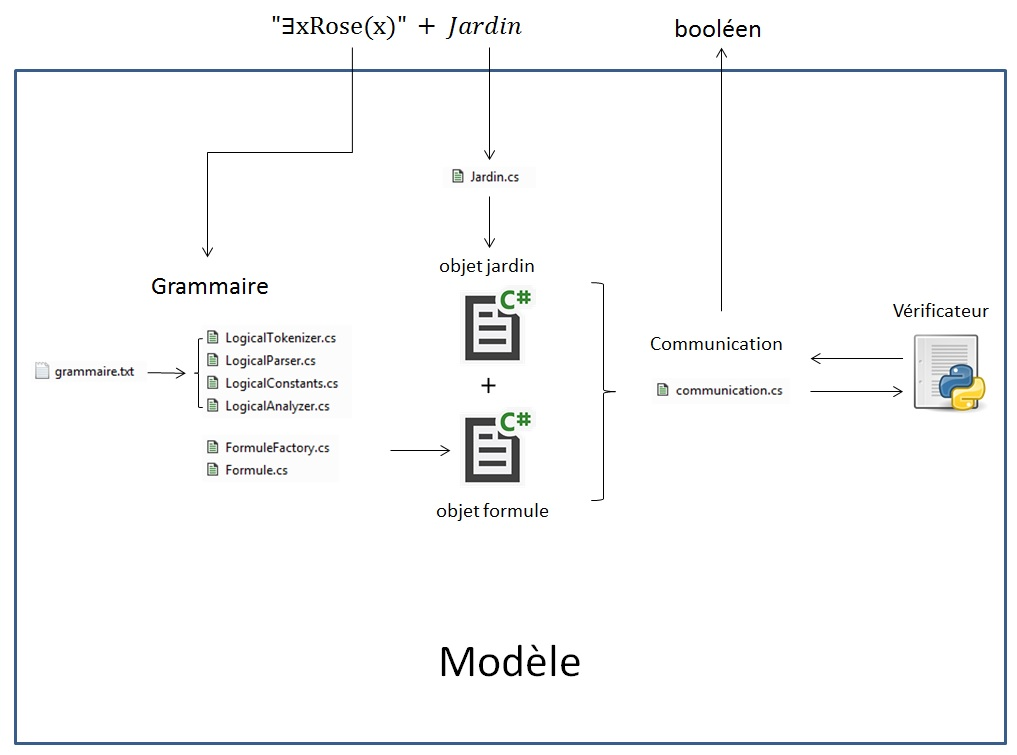
\includegraphics[scale=0.35]{communication}
	\end{frame}
	
	\section{Objectifs pour les prochaines semaines}
	\begin{frame}
	\begin{itemize}
		\setlength\itemsep{2em}
		\item Modélisation du plateau et des objets 3D
		\item Création du clavier visuel et du formulaire de saisie de formule
		\item Test approfondis du traitement de vérification de formule
	\end{itemize}
	\end{frame}
	
\end{document}

\chapter{Analyse de l'existant}

Le projet tourne autour d'un script préalablement fourni en python.

\section{Script python}

Le script permet de créer un jardin en disposant les différents éléments avec leurs attributs sur diverses coordonnées.
En premier lieu il est nécessaire de bien créer un jardin, il serait inutile de tester une formule sans contexte autour.
Le script permet ensuite de créer une formule, celle-ci doit être préalablement vérifiée pour que sa syntaxe ne contienne aucun erreur.
Dans un dernier temps le script analyse la formule dans le contexte du jardin donné et retourne un booléen en résultat.


\section{Bilan récapitulatif}

Voici le tableau (cf. fig. 2.1) récapitulatif de l'analyse de l'existant:\\

%tableau centré à taille variable qui s'ajuste automatiquement suivant la longueur du contenu
\begin{figure}[!h]
\begin{center}
\begin{tabular}{|l|l|l|l|}
  \hline
  Solution & Création & Vérification & Analyse\\
  \hline
  Jardin & Oui & Non & Non \\
  Formule & Oui & Non & Oui \\
  \hline
\end{tabular}
\end{center}
\caption{Tableau récapitulatif des solutions}
\end{figure}

 
\chapter{Analyse des besoins}

Le projet s'axe sur le besoin fonctionnel de base de l'interface graphique autour duquel gravitent des besoins non fonctionnels mais nécessaires au bon fonctionnement de l'application.

\section{Besoins}

Après une analyse des besoins du projet, nous avons défini deux sous catégories. D'un côté, les besoins graphiques, de l'autre, les besoins liés à la syntaxe des formules.

\subsection{Interface Graphique}

L'interface graphique doit être ergonomique et \textit{user-friendly}, le but est d'accompagner les étudiants dans l'apprentissage de la logique du premier ordre de la manière la plus agréable possible. Pour cela un certain nombre d'exigences en terme de GUI ont été mis en place:

\begin{itemize}
\item un jardin représenté par une grille de taille fixe;
\item des fleurs pouvant être disposées sur le jardin et ayant un visuel différent selon leurs espèces, tailles et couleurs;
\item un menu permettant de positionner de nouvelles fleurs à la souris et d’en changer les caractéristiques;
\item  un menu permettant d’écrire et vérifier des formules de la logique du premier ordre à l’aide d’un clavier virtuel et d’une liste de 5 variables et de 20 constantes;
\item  un menu permettant de sélectionner une variable ou une constante;
\item  un clavier visuel permettant de sélectionner les connecteurs de la logique (not, et, ou, pour tout, etc.);
\item  un menu permettant de sauvegarder et de charger des jardins et/ou des ensembles de formules.
\end{itemize}

Aperçu du rendu souhaité :

\begin{figure}[!h]
\begin{center}
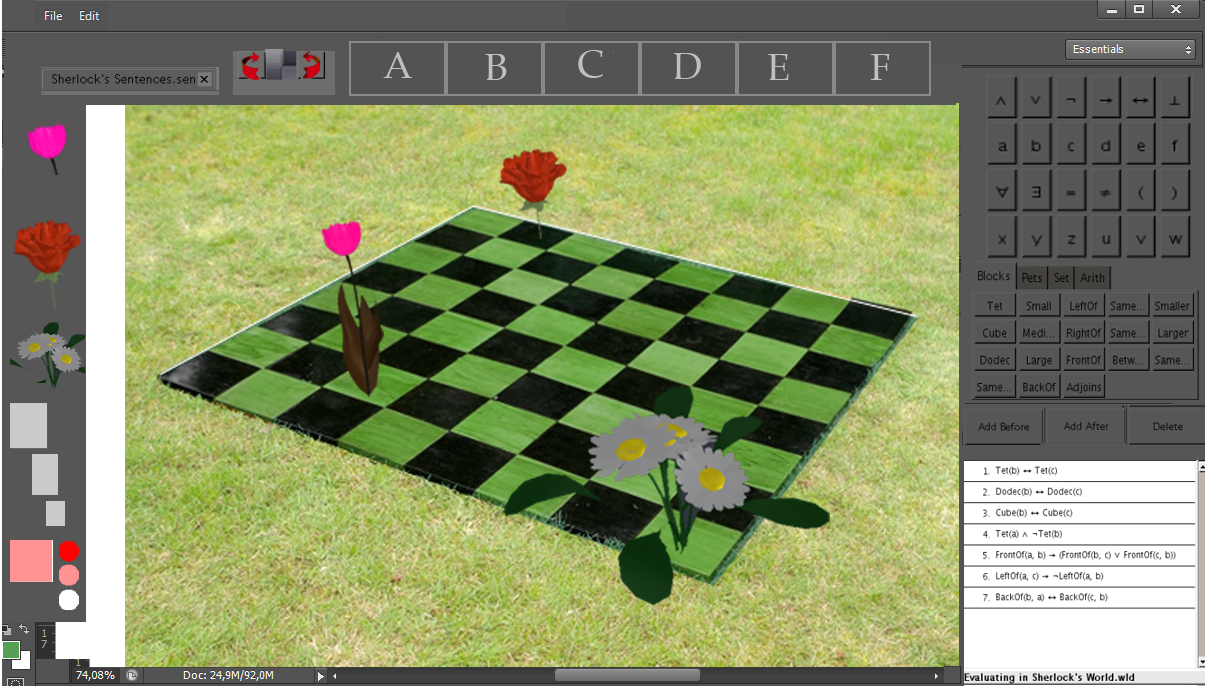
\includegraphics[height=10cm]{besoins/simulation.png}
\end{center}
\caption{Rendu attendu}
\end{figure}

\clearpage


\subsection{Analyse Syntaxique}

L'analyse syntaxique est un besoin lié directement au script fourni avec le sujet du projet. Si cette partie n'est pas parfaitement fonctionnelle, le script ne pourra donc pas fonctionner correctement et le projet ne pourra aboutir.\\
Idéalement, dans le cas d'une formule syntaxiquement fausse, l'analyseur pourra indiquer ou se trouve l'erreur dans la formule entrée par l'utilisateur. Cependant ce point n'est pas une nécessité, cette partie doit en priorité stopper le programme et notifier l'utilisateur du non respect de la syntaxe dans l'une de ses formules.\\

Il n'est utile d'aborder qu'un seul besoin non-fonctionnel: la communication entre deux langages différents, ce point étant technique nous préférons revenir dessus plus tard et seulement l'évoquer ici.
Il a cependant été pris en compte les contraintes de développement,  détaillées à la fin de cette partie.


\section{Développement}

Le développement est réparti en tâches parallélisées afin d'optimiser le temps de réalisation.

\subsection{Tâches}

Le développement s'axe sur trois grandes tâches, la communication inter langages, l'analyse syntaxique et la création de l'interface graphique. Le but étant de relier les trois blocs ensemble pour obtenir l'application finale.

%tableau à taille fixée sur certaines colonnes (param sur la ligne \begin{tabularx}, voir wiki pour plus d'info sur la syntaxe
\begin{figure}[!h]
\begin{center}
\begin{tabularx}{17cm}{|c|p{6cm}|X|}
  \hline
  Priorité & Nom & Raison\\
  \hline
  1 & Communication inter langages & Doit être vérifié en premier car sinon on ne pourra pas utiliser l'Analyseur Syntaxique \tabularnewline
  2 & Analyseur Syntaxique & On doit pouvoir entrer n'importe quel formule et être capable de détecter au plus vite la moindre erreur dans celle-ci \tabularnewline
  3 & Liaison Communication-Analyseur & Comme les principales fonctionnalités permettant de tester sont opérationnelles, nous pouvons passer à cette tâche. \tabularnewline
  4 & Création de l'interface graphique & Dernière fonctionnalité essentielle à mettre en place. \tabularnewline
  5 & Animation des fleurs & Non-essentiel, mais apporterait un plus au projet. \tabularnewline
  6 & Fonctionnalité de retour en arrière & Non-essentiel, mais apporterait un plus au projet. \tabularnewline
  \hline
\end{tabularx}
\end{center}
\caption{Tableau récapitulatif des tâches}
\end{figure}

\subsection{Organisation du code}

Dans le cas où l'analyseur syntaxique détecterait une erreur de formule, celui-ci ne retournera pas d'objets mais notifiera le bloc de communication de l'erreur. Ce dernier remontera donc le soucis au bloc GUI qui l'affichera à l'utilisateur.

\begin{figure}[!h]
\begin{center}
\includegraphics[height=10cm]{besoins/organisationProg.png}
\end{center}
\caption{organisation des blocs}
\end{figure}


\input{./autre_partie.tex}

\chapter{Résultats}

Pour conclure il est de mise de faire un état des fonctionnalités finales du programme et de les comparer à ce qui était attendu initialement.

\section{Évolution des fonctionnalités}

Les objectifs concernant l'analyse syntaxique et la communication avec le script de base ont bien été atteints conformément aux pré-requis établis pour pouvoir avoir une interface graphique fonctionnelle. \\
Cependant nous avons du ajuster quelques technologies choisies lors de la réalisation du cahier des charges. Comme évoqué dans le chapitre 3.1.2 sur la Communication avec le script Python, nous avions à l'origine choisi de faire la liaison avec un script Ocaml qui s'est avéré être trop compliquée à mettre en place.
\\
Concernant l'interface graphique, de nombreux points avaient été mis en avant lors de la réalisation du cahier des charges et rappelés dans les chapitres précédents (voir chapitre 2.1 Besoins). Tous les objectifs principaux ont été atteints. Lors de l'avancée du projet, nous avions prévu de faire un système de \textit{Drag \& Drop} depuis un panel vers le jardin (voir chapitre 3.2.3 Le Jardin et les fleurs), nous avons du revoir nos exigences à la baisse devant le temps de programmation restant.
\\
Nous avons d'ailleurs, et ce tout du long de ce projet, tenu nos engagements par rapport au diagramme de Gantt fixé dans le cahier des charges (voir annexes). Bien que nous ayons espéré finir plus tôt afin de pouvoir ajouter des fonctionnalités supplémentaires.
\newline Dans les causes de petit retards, initialement pris en compte dans la réalisation du planning, on pourra noter la perte de temps avec le premier script Ocaml, les soucis avec GitHub qui bloque les commit de trop grande taille, le passage à un git sur un serveur privé qu'il a fallut monter nous même et donc impliquant des petits soucis de configuration à ajuster et enfin la configuration de Unity à ajuster pour pouvoir y faire passer des librairies externes.
\\
Toutes les fonctionnalités principales nécessaires pour le bon fonctionnement et la bonne utilisation du logiciel sont donc opérationnelles. Mais il est bien entendu toujours possible d'apporter de nouvelles améliorations aussi bien graphiques (améliorer et personnaliser l'aspect graphique de l'interface, création de nouveaux environnements, etc.) que fonctionnelles (ajouter un outil de "retour en arrière", permettre à l'utilisateur de définir des raccourcis pour l'utilisation du clavier, etc.).



\chapter{Bilan}

%Rappel du context
Intro / Rappel Contexte

Nous avons donc pu en tirer la problématique suivante :

\begin{center}
\hskip7mm
Problématique du sujet
\end{center}



%Rappel des résultats


\newpage

%Conclusion/Perspectives


%Ne pas numéroter cette partie
\part*{Annexes}
%Rajouter la ligne "Annexes" dans le sommaire
\addcontentsline{toc}{part}{Annexes}

\begin{center}\textbf{Vocabulaire}\end{center}

\begin{itemize}
\item \textsc{Panel}: Élément graphique de Unity 5 représenté par un panneau configurable sur lequel placer des éléments héritant de la classe UI.
\item \textsc{UI}: \textit{User Interface}, classe fournie par Unity comprenant les Panels, boutons, textes, éléments d'interface graphique. 
\item \textsc{Drag \& Drop}: Glisser-déposer en français, manière de gérer une interface en permettant le déplacement de certains éléments vers d'autres conteneurs. 
\item \textsc{Tile}: Tuile en français, correspond à une case du jardin.
\end{itemize}

\begin{center}\textbf{Grammaire pour la vérification syntaxique}\end{center}

\begin{center}
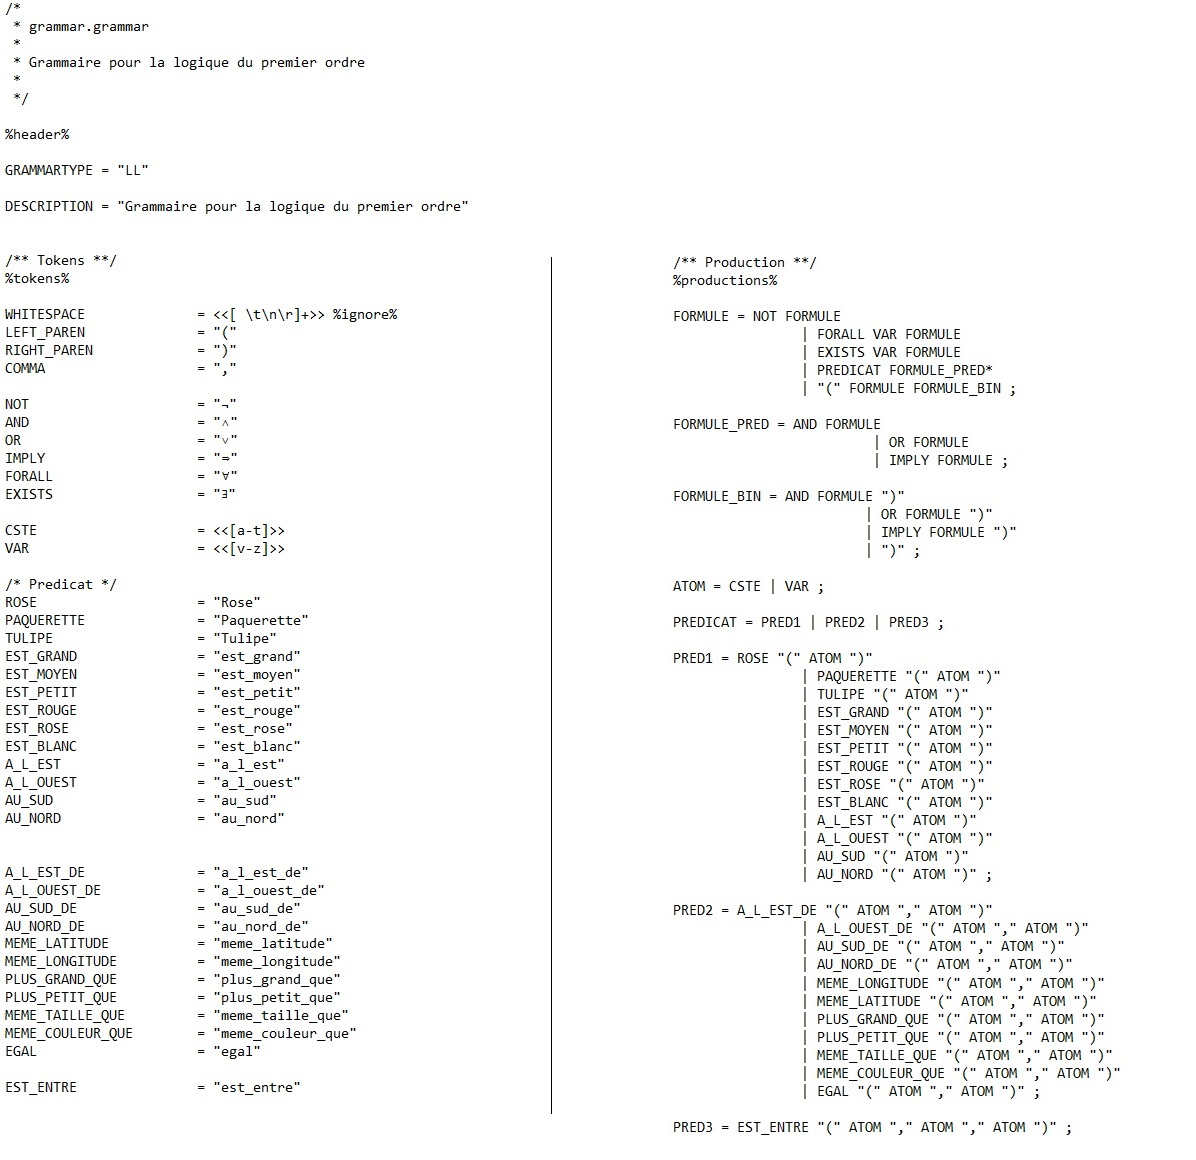
\includegraphics[scale=0.5]{annexes/grammaire.jpg}
\end{center}

\newpage

%récupérer les citation avec "/footnotemark"
\nocite{*}

%choix du style de la biblio
\bibliographystyle{plain}
%inclusion de la biblio
\bibliography{bibliographie.bib}
%voir wiki pour plus d'information sur la syntaxe des entrées d'une bibliographie

\end{document}